\documentclass[a4paper,12pt]{article}
\usepackage[utf8]{inputenc}
\usepackage[spanish]{babel}
\usepackage{graphicx}
\usepackage{anysize}
\marginsize{3cm}{3cm}{1cm}{1cm} 
\usepackage{cite}

\begin{document}

\title{ Las 7 Maravillas del Mundo}
\author{Adrián Béjar González}
\date{Enero 2016}
\maketitle

Presentación de las Siete Maravillas del Mundo ganadoras en una votación 

\section{Asia}
 \subsection{Petra}
Petra es un importante enclave arqueológico en Jordania, y la capital del antiguo reino nabateo. El nombre de Petra proviene del griego con el significado de piedra, y su nombre es perfectamente idóneo; no se trata de una ciudad construida con piedra sino, literalmente, excavada y esculpida en la piedra.

El asentamiento de Petra se localiza en un valle angosto, al este del valle de la Aravá que se extiende desde el mar Muerto hasta el Golfo de Aqaba. Los restos más célebres de Petra son sin duda sus construcciones labradas en la misma roca del valle (hemispeos), en particular, los edificios conocidos como el Khazneh (el Tesoro) y el Deir (el Monasterio).

Fundada en la antigüedad hacia el final de siglo VIII a. C. por los edomitas, fue ocupada en el siglo VI a. C. por los nabateos que la hicieron prosperar gracias a su situación en la ruta de las caravanas que llevaban el incienso, las especias y otros productos de lujo entre Egipto, Siria, Arabia y el sur del Mediterráneo.

Hacia el siglo VI d. C., el cambio de las rutas comerciales y los terremotos sufridos, condujeron al abandono de la ciudad por sus habitantes. Cayó en el olvido hasta que en 1812 el lugar fue redescubierto para el mundo occidental por el explorador suizo Jean Louis Burckhardt (1784-1817).

Numerosos edificios cuyas fachadas están directamente esculpidas en la roca, forman un conjunto monumental único, que a partir del 6 de diciembre de 1985 está inscrito en la Lista del Patrimonio Mundial de la Unesco. La zona que rodea el lugar es también, desde 1993, Parque Nacional arqueológico.

Desde el 7 de julio de 2007, Petra forma parte de las Las nuevas siete maravillas del mundo moderno.
 \subsection{Gran Muralla China}  
La Gran Muralla China es una antigua fortificación china construida y reconstruida entre el siglo V a. C. y el siglo XVI (Edad Moderna) para proteger la frontera norte del Imperio chino durante las sucesivas dinastías imperiales de los ataques de los nómadas xiongnu de Mongolia y Manchuria.

Contando sus ramificaciones y construcciones secundarias, se calcula que tiene 21 196 kilómetros de largo, desde la frontera con Corea, al borde del río Yalu, hasta el desierto de Gobi, a lo largo de un arco que delinea aproximadamente el borde sur de Mongolia Interior, aunque hoy solo se conserva un 30% de ella.3 En promedio, mide de 6 a 7 metros de alto y de 4 a 5 metros de ancho.

La muralla fue designada Patrimonio de la Humanidad por la Unesco en el año 1987. Gran parte de la Gran Muralla tiene fama de ser el mayor cementerio del mundo. Aproximadamente 10 millones de trabajadores murieron durante su construcción.4 No se los enterró en el muro en sí, sino en sus inmediaciones.

El día 26 de enero de 2007 se dio a conocer que la muralla china fue elegida como una de las ganadoras en la lista de Las Nuevas Siete Maravillas del Mundo Moderno.
 \subsection{Taj Mahal} 
 El Taj Mahal es un complejo de edificios construido entre 1631 y 1648 en la ciudad de Agra, estado de Uttar Pradesh (India), a orillas del río Yamuna, por el emperador musulmán Shah Jahan de la dinastía mogola. El imponente conjunto se erigió en honor de su esposa favorita, Arjumand Bano Begum —más conocida como Mumtaz Mahal— que murió en el parto de su decimocuarta hija. Se estima que su construcción necesitó el esfuerzo de unos 20 000 obreros.

El Taj Mahal es considerado el más bello ejemplo de arquitectura mogola, estilo que combina elementos de las arquitecturas islámica,1 persa,2 india e incluso turca.3 Este monumento ha logrado especial notoriedad por el carácter romántico de su inspiración. Aunque el mausoleo cubierto por la cúpula de mármol blanco es la parte más conocida, el Taj Mahal es un conjunto de edificios integrados.

El monumento es un importante destino turístico de la India. En 1983, fue reconocido por la Unesco como Patrimonio de la Humanidad, y nombrado una de Las Nuevas Siete Maravillas del Mundo Moderno.
\section{Europa} 
 \subsection{Coliseo de Roma}
 El Coliseo (en latín: Amphitheatrum Flavium Romae) es un anfiteatro de la época del Imperio romano, construido en el siglo I d.C. y ubicado en el centro de la ciudad de Roma. Originalmente era denominado Anfiteatro Flavio (Amphitheatrum Flavium), en honor a la Dinastía Flavia de emperadores que lo construyó, y pasó a llamarse Colosseum por una gran estatua que había cerca, el Coloso de Nerón, que no ha llegado hasta nosotros. Por su conservación e historia, el Coliseo es uno de los monumentos más famosos de la antigüedad clásica. Fue declarado Patrimonio de la Humanidad en 1980 por la Unesco y una de Las Nuevas Siete Maravillas del Mundo Moderno el 7 de julio de 2007.

En la antigüedad poseía un aforo para unos 12 000 espectadores, con ochenta filas de gradas.1 2 3 Los que estaban cerca de la arena eran el Emperador y los senadores, y a medida que se ascendía se situaban los estratos inferiores de la sociedad. En el Coliseo tenían lugar luchas de gladiadores y espectáculos públicos. Se construyó justo al este del Foro Romano, y las obras empezaron entre 70 d. C. y 72 d. C., bajo el mandato del emperador Vespasiano. El anfiteatro, que era el más grande jamás construido en el Imperio romano, se completó en 80 d. C. por el emperador Tito, y fue modificado durante el reinado de Domiciano.4 Su inauguración duró 100 días, participando en ella todo el pueblo romano y muriendo en su celebración decenas de gladiadores y fieras que dieron su vida por el placer y el espectáculo del pueblo.4

El Coliseo se usó durante casi 500 años, celebrándose los últimos juegos de la historia en el siglo VI, bastante más tarde de la tradicional fecha de la caída del Imperio romano de Occidente en 476 d. C. Los bizantinos también lo utilizaron durante el siglo VI. Además de las peleas de gladiadores, muchos otros espectáculos públicos tenían lugar aquí, como naumaquias, caza de animales, ejecuciones, recreaciones de famosas batallas y obras de teatro basadas en la mitología clásica. El edificio dejó de emplearse para estos propósitos en la Alta Edad Media. Más tarde, sirvió como refugio, fábrica, sede de una orden religiosa, fortaleza y cantera. De sus ruinas se extrajo abundante material para la construcción de otros edificios, hasta que fue convertido en santuario cristiano, en honor a los cautivos martirizados durante los primeros años del cristianismo. Esta medida contribuyó a detener su expolio y a que se conservara.

Aunque la estructura está seriamente dañada debido a los terremotos y los picapedreros, el Coliseo siempre ha sido visto como un icono de la Roma Imperial y es uno de los ejemplos mejor conservados de la arquitectura romana. Es una de las atracciones turísticas más populares de la moderna Roma y aún está muy ligado a la Iglesia católica romana, por lo que el papa encabeza el viacrucis hasta el anfiteatro cada Viernes Santo.
\section{América}
 \subsection{Cristo Redentor}
 El Cristo Redentor o Cristo de Corcovado es una estatua de 38 metros, con el pedestal de 8 metros, de Jesús de Nazaret con los brazos abiertos mostrando a la ciudad de Río de Janeiro, en Brasil. Está situada a 710 metros sobre el nivel del mar en el Parque Nacional de la Tijuca, en la cima del cerro del Corcovado. Fue inaugurado el 12 de octubre de 1931, después de aproximadamente cinco años de obras.
 \subsection{Machu Pichu}
Machu Picchu (del quechua sureño machu pikchu, «Montaña Vieja») es el nombre contemporáneo que se da a una llaqta —antiguo poblado andino— incaica construida a mediados del siglo XV en el promontorio rocoso que une las montañas Machu Picchu y Huayna Picchu en la vertiente oriental de la cordillera Central, al sur del Perú y a 2490 msnm, altitud de su plaza principal. Su nombre original habría sido Picchu o Picho.1

Según documentos de mediados del siglo XVI,2 Machu Picchu habría sido una de las residencias de descanso de Pachacútec, noveno inca del Tahuantinsuyo entre 1438 y 1470. Sin embargo, algunas de sus mejores construcciones y el evidente carácter ceremonial de la principal vía de acceso a la llaqta demostrarían que esta fue usada como santuario religioso.3 Ambos usos, el de palacio y el de santuario, no habrían sido incompatibles. Algunos expertos parecen haber descartado, en cambio, un supuesto carácter militar, por lo que los populares calificativos de «fortaleza» o «ciudadela» podrían haber sido superados.4

Machu Picchu es considerada al mismo tiempo una obra maestra de la arquitectura y la ingeniería.5 Sus peculiares características arquitectónicas y paisajísticas, y el velo de misterio que ha tejido a su alrededor buena parte de la literatura publicada sobre el sitio, lo han convertido en uno de los destinos turísticos más populares del planeta.6

Machu Picchu está en la Lista del Patrimonio de la Humanidad de la Unesco desde 1983, como parte de todo un conjunto cultural y ecológico conocido bajo la denominación Santuario histórico de Machu Picchu. El 7 de julio de 2007 Machu Picchu fue declarada como una de las nuevas siete maravillas del mundo moderno en una ceremonia realizada en Lisboa, Portugal, que contó con la participación de cien millones de votantes en el mundo entero.
 \subsection{Chichén Itzá}
Chichén Itzá es uno de los principales sitios arqueológicos de la península de Yucatán, en México, ubicado en el municipio de Tinum, en el estado de Yucatán. Vestigio importante y renombrado de la civilización maya, las edificaciones principales que ahí perduran corresponden a la época de la declinación de la propia cultura maya denominada por los arqueólogos como el período posclásico.

La arquitectura monumental que ha llegado hasta nuestros días, que es emblemática del yacimiento, tiene una clara influencia tolteca. El dios que preside el sitio, según la mitología maya, es Kukulcán, representación maya de Quetzalcóatl, dios tomado del panteón de la cultura tolteca.

Chichén Itzá fue una ciudad o un centro ceremonial, que pasó por diversas épocas constructivas e influencias de los distintos pueblos que la ocuparon y que la impulsaron desde su fundación.

La zona arqueológica de Chichén Itzá fue inscrita en la lista del Patrimonio de la Humanidad por la Unesco en 1988.3 El 7 de julio de 2007, el Templo de Kukulcán, ubicado en Chichén Itzá, fue reconocido como una de las Las nuevas siete maravillas del mundo moderno, por una iniciativa privada sin el apoyo de la Unesco, pero con el reconocimiento de millones de votantes alrededor del mundo.
 \\

\begin{bf} 
Nominadas en España:
\end{bf} 

\begin{enumerate}
 \item Alhambra
 \item Templo de la Sagrada Familia
 \item Santiago de Compostela
 \item La Giralda
 \item Mezquita de Córdoba
 \item Museo Guggenheim Bilbao
 \item Palacio Real de Madrid
 \item Acueducto de Segovia
\end{enumerate}


\begin{figure}[h]
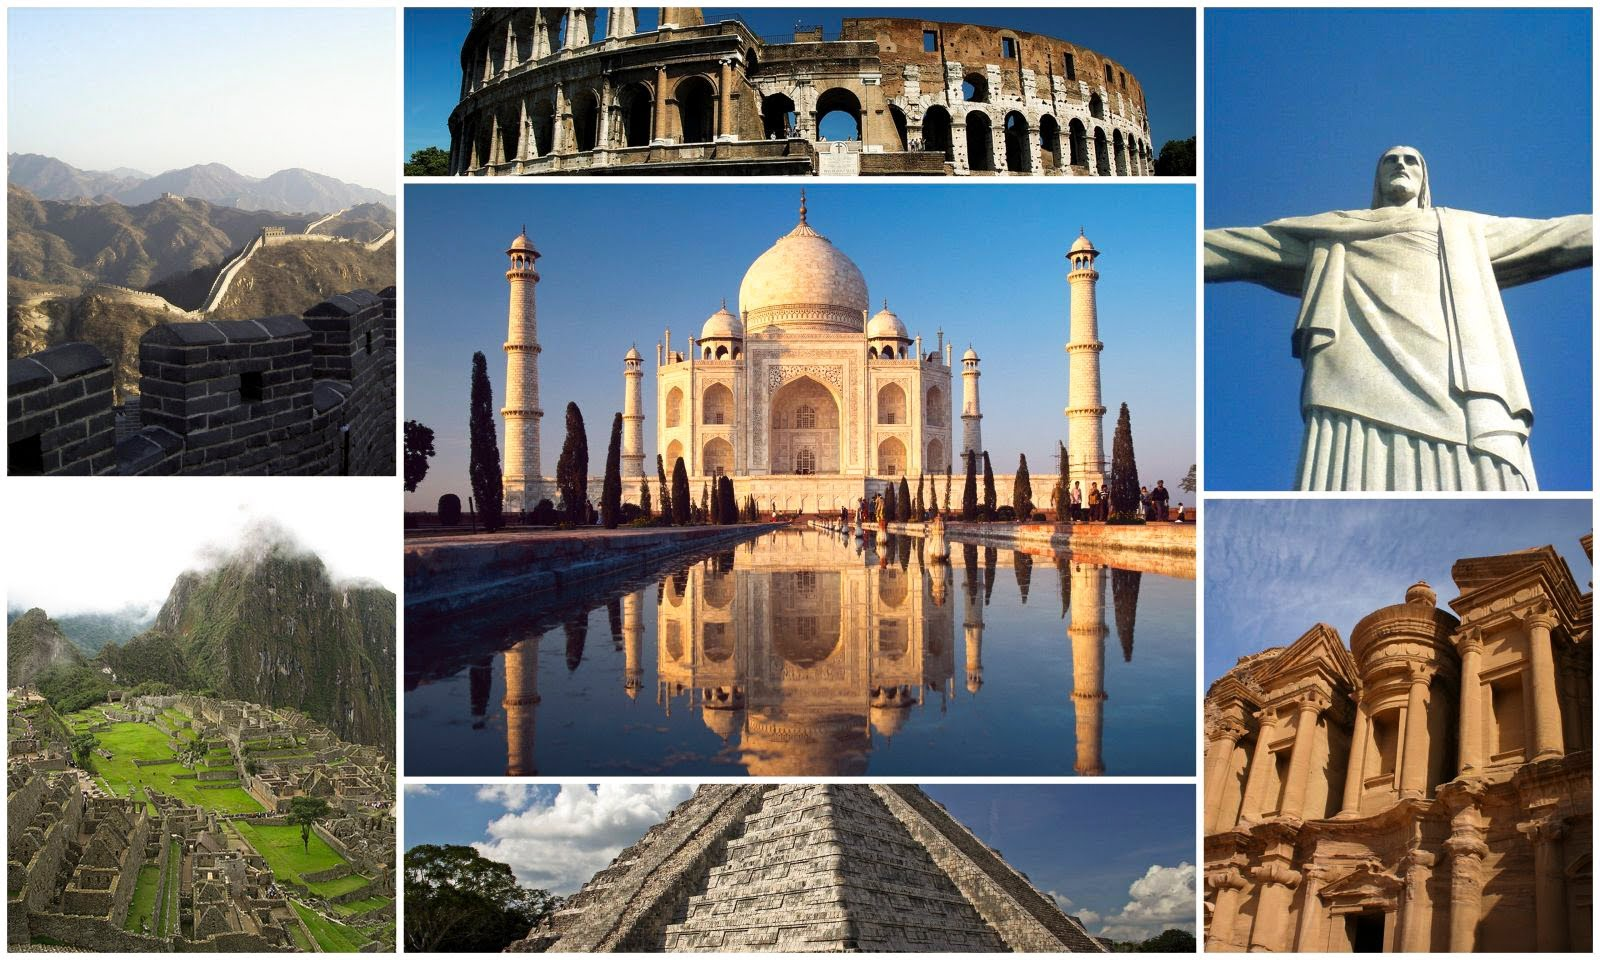
\includegraphics[width=1\textwidth]{maravillas}
\caption{Mix Maravillas}
\label{blanco}
\end{figure}


\begin{bf} 
Fórmula Matemática más Bella - Fórmula de Euler:
\end{bf} 

\begin{equation}
e^{i\pi}+1=0
\end{equation}\\

\begin{bf} 
Maravillas y Año de Inscripción
\end{bf}\\ 

\begin{tabular}{|c|c|c|c|c|c|c|}
\hline 
Chichén Itzá & Coliseo de Roma & Cristo Redentor & Gran Muralla China & Machu Picchu & Petra & Taj Mahal \\ 
\hline 
1988 & 1990 & 2007 & 1987 & 1983 & 1985 & 1983 \\ 
\hline 
\end{tabular}\\ \\

\bibliographystyle{acm}
\bibliography{Biblio}

\cite{CoxMorris2000}

\end{document} 


